\documentclass[slovene,11pt,a4paper]{article}
\usepackage[margin=1.8cm,bottom=3cm,foot=1.5cm]{geometry}
\usepackage{amsmath}
\usepackage{booktabs}
\usepackage{float}
\usepackage{graphicx}
\usepackage{changepage}
\usepackage{subcaption}
\usepackage{multirow}
\usepackage{blindtext}
\usepackage{hyperref}
\usepackage[version=4]{mhchem}
\usepackage[slovene]{babel}
\pagenumbering{gobble}

\begin{document}

\title{Zaključna naloga - Radioterapija}
\author{Tadej Lozej 28242023}
\maketitle

\begin{center}
Modelska analiza 1 \\
\bigskip
Predavatelj: prof. dr. Simon Širca \\
Asistent: doc. dr. Miha Mihovilovič
\end{center}

\newpage

\tableofcontents

\newpage

\pagenumbering{arabic}

\section{Navodilo naloge}

V radioterapiji je poglavitni problem načrtovanje doze obsevanja. Izvire sevanja je treba razporediti tako, da v predelih tumorja zagotovijo dozo, ki je večja od kritične doze za uničenje tkiva, v zdravem okoliškem tkivu pa naj bo prejeta doza čim manjša. Postavili bomo najpreprostejši 2D model: obsevanje z vzporednim snopom sevanja, ki ga enakomerno pomikamo prek tarče v dveh pravokotnih smereh. Pojemanje žarka v tkivu z globino zanemarimo.

Na sliki \ref{fig:tumor} je tumorsko področje smo označili senčeno, ostalo je zdravo tkivo. Puščice pomenijo posamezne diskretizirane snope sevanja. V gornji sliki je 6 × 7 = 42 celic, neznane količine so jakosti 6 + 7 = 13 curkov. Vsaka celica prejme dozo, ki je vsota jakosti obeh curkov, ki se v njej križata. Za celice tumorja zahtevamo, da je ta vsota večja od kritične (ki jo uporabimo za enoto), za zdrave pa zahtevamo, da je njihova skupna prejeta doza čim manjša.

\begin{figure}[h!]
\centering
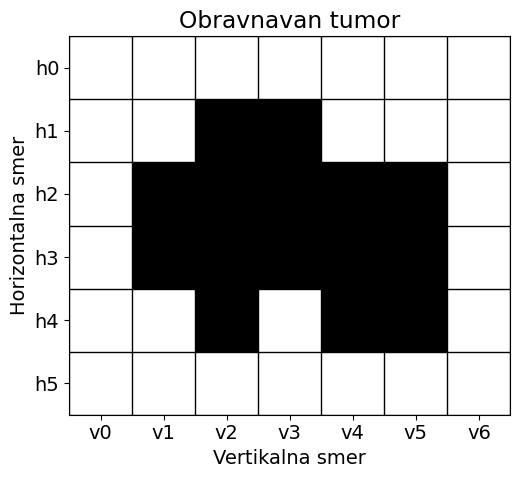
\includegraphics[width=9cm]{tumor.png}
\caption{Senčeno je prikazan tumor. V horizontalni smeri imamo 6 kanalov po katerih lahko tumor obsevamo, v vertikalni pa 7.}
\label{fig:tumor}
\end{figure}

V duhu linearnega programiranja je tudi obratna formulacija (ki pa manj ustreza radiološkim zahtevam): v vsaki od zdravih celic naj bo prejeta doza manjša od enote, skupna doza v tumorskih celicah pa čim večja. Eksperimentiraš lahko še s preprostejšimi obsevalnimi polji ali pa tudi z bolj zahtevnimi, ki terjajo več snopov in s tem več spremenljivk.

\section{Uvod}

Nalogo bomo rešili s pomočjo linearnega programiranja. To lahko storimo, ker je doza sevanja $D_{ij}$ v vsaki celici linearno odvisna od jakosti curkov. Doza, ki jo prejme posamezna celica, je enaka vsoti prispevkov horizontalnega in vertikalnega curka

\begin{equation}
D_{ij} = H_i + V_j,
\end{equation}
kjer sta $H_i$ in $V_j$ jakosti curkov v $i$-tem horizontalnem oziroma $j$-tem vertikalnem kanalu. K postavitvi linearnega problema lahko pristopimo na dva načina, kot je opisano v navodilih naloge.

\subsection{Minimizacija doze v zdravem tkivu}

Prvi pristop je minimizacija doze v zdravem tkivu, ob pogoju, da tumorske celice prejmejo vsaj kritično dozo, ki jo v našem modelu postavimo enako 1. Označimo z $\vec{c}$ vektor, katerega komponente predstavljajo število zdravih celic v posameznih vrsticah in stolpcih. Na primer, za tumor iz slike \ref{fig:tumor} dobimo

\[
\vec{c} = (7, 5, 2, 2, 4, 7, 6, 4, 2, 3, 3, 3, 6),
\]
saj je v prvi vrstici 7 zdravih celic, v drugi 5, itd. Od sedme komponente vektorja dalje drugi nadaljujemo s stolpci. Iskani vektor $\vec{x}$ predstavlja jakosti vseh žarkov

\[
\vec{x} = (H_0, H_1, H_2, \ldots, H_5, V_0, V_1, \ldots, V_6).
\]

Namen je minimizirati skupno dozo v zdravem tkivu $D^{\text{(zdravo tkivo)}}$, kar ustreza skalarnemu produktu

\begin{equation}
D_{\text{min}}^{\text{(zdravo tkivo)}} = \min(\vec{c} \cdot \vec{x}).
\end{equation}
Pogoj, ki ga moramo upoštevati, je, da mora biti vsota prispevkov žarkov v tumorskih celicah vsaj enaka kritični dozi. To zapišemo z neenačbo

\begin{equation}
A_{\text{lb}} \vec{x} \geq \vec{b}_{\text{lb}},
\end{equation}
kjer je $A_{\text{lb}}$ matrika velikosti (število tumorskih celic) × (število curkov), ki določa kateri jakosti žarkov se morata sešteti vsaj v vrednost, ki jo določa ustrezna komponenta $b_{lb}$. V našem primeru je $A$ dimenzij 15 × 13, vektor $\vec{b}_{\text{lb}}$ pa vsebuje petnajst enic — kritična doza v vsaki tumorski celici. Ker funkcija \texttt{scipy.optimize.linprog} podpira le zgornje meje, neenačbo pomnožimo z $-1$.

\subsection{Maksimizacija doze v tumornem tkivu}

Drugi pristop je maksimizacija skupne doze v tumorskih celicah, ob pogoju, da v zdravih celicah ne presežemo kritične doze (v našem primeru vrednosti 1). V tem primeru vektor $\vec{c}$ vsebuje število tumorskih celic v posameznih vrsticah in stolpcih.

Ker \texttt{linprog} rešuje probleme minimizacije, maksimizacijo enostavno preoblikujemo

\begin{equation}
D_{\text{max}}^{\text{(tumorno tkivo)}} = \max(\vec{c} \cdot \vec{x}) = \min(-\vec{c} \cdot \vec{x}).
\end{equation}
Pogoj za zdrave celice je

\begin{equation}
A_{\text{ub}} \vec{x} \leq \vec{b}_{\text{ub}},
\end{equation}
kjer je $A_{\text{ub}}$ matrika velikosti (število zdravih celic) × (število curkov), vektor $\vec{b}_{\text{ub}}$ pa vsebuje 27 enic — zgornjo mejo za prejeto dozo v vsaki zdravi celici. V našem primeru je matrika $A$ dimenzij 27 × 13.

\section{Model konstantnega curka}

Na spodnjih dveh slikah si poglejmo rešitvi za obravnavan tumor. Tumor je na obeh slikah prikazan z črno obrobo in šrafuro. Doza, ki jo vsaka celica prejme je prikazana z gradientom rdeče barve. Prav tako je količina doze na vsaki celici zapisana z modro številko. Na sliki \ref{fig:doze_sevanja_1} vidimo rešitev dobljeno z minimizacijo doze v zdravem tkivu. Tumor je obsevan iz treh horizontalnih kanalov in dveh vertikalnih kanalov. Vse tumorne celice prejmejo višjo dozo sevanja kot je kritična doza. Nekaj zdravih celic prav tako prejme višjo dozo kot kritično dozo. Na sliki \ref{fig:doze_sevanja_2} pa vidimo rešitev dobljeno z maksimizacijo doze v tumorju. Vidimo, da v tem primeru tumorno tkivo prejme višjo dozo sevanja kot v prejšnjem primeru. A prav tako prejme večjo skupno dozo tudi zdravo tkivo. V tabeli \ref{tab:doze_sevanja} lahko vidimo skupno prejeto dozo in povprečno dozo na celicu v zdravem in tumornem tkivu pri obeh načinih reševanja linearnega problema.

\begin{figure}[h!]
\centering
\includegraphics[width=12cm]{doze_sevanja_1.png}
\caption{Rešitev pridobljena z minimizacijo doze sevanja v zdravem tkivu. Tumor je obrobljen z črno in čez njega je šrafura. Doza, ki jo prejmejo posamezne celice je prikazana z rdečo barvo in modrim napisom.}
\label{fig:doze_sevanja_1}
\end{figure}

\begin{figure}[h!]
\centering
\includegraphics[width=12cm]{doze_sevanja_2.png}
\caption{Rešitev pridobljena z maksimizacijo doze sevanja v tumornem tkivu. Tumor je obrobljen z črno in čez njega je šrafura. Doza, ki jo prejmejo posamezne celice je prikazana z rdečo barvo in modrim napisom.}
\label{fig:doze_sevanja_2}
\end{figure}

\begin{table}[h!]
\centering
\begin{tabular}{c|c|c||c|c|}
\cline{2-5}		
		& \multicolumn{2}{c||}{Zdravo tkivo} & \multicolumn{2}{c|}{Tumorno tkivo} \\
\cline{2-5}
		& Skupna doza & Povprečna doza & Skupna doza & Povprečna doza \\
\hline
Način 1	& 13 & 0,48 & 20 & 1,33 \\
Način 2	& 19 & 0,70 & 25 & 1,67 \\
\hline
\end{tabular}
\caption{Skupna in povprečna doza na celico v zdravem in tumornem tkivu pri minimizaciji doze v zdravem tkivu (Način 1) ter maksimizaciji doze v tumorju (Način 2).}
\label{tab:doze_sevanja}
\end{table}

\subsection{Porazdelitev doz sevanja v 15 celičnem tumorju}

Obravnavani tumor je velikosti 15 celic in je določene oblike. Vprašajmo se kakšna je porazdelitev prejetih doz zdravih celic in tumornih celic pri tumorju velikemu 15 celic. Na sliki \ref{fig:nakljucni_tumorji} lahko vidimo nekaj naključno generiranih tumorjev velikosti 15 celic. Pri tej obravnavi zanemarjamo dejstvo, da se tumorne celice običajno držijo v skupku. Zaradi tega lahko pričakujemo višje doze v zdravem tkivu.

\begin{figure}[h!]
\centering
\includegraphics[width=\linewidth]{nakljucni_tumorji.png}
\caption{Štirje naključni tumorji velikosti 15 celic. Tumorne celice so prikazane s črno barvo.}
\label{fig:nakljucni_tumorji}
\end{figure}

Na sliki \ref{fig:porazdelitev_doz_zdravih_celic} lahko vidimo porazdelitev doz, ki jih prejmejo zdrave celice v tisoč različnih tumorjih velikosti petnajst celic. Na grafu sta prikazana oba načina reševanja linearnega problema. Način 1 se nanaša na minimizacijo sevanja v zdravem tkivu, način 2 pa na maksimizacijo sevanja v tumornem tkivu. Na grafu vidimo, da v načinu 2 nobena zdrava celice ne prejme doze večje od kritične doze, kar je seveda določeno s pogojem. Na grafu sta desno zgoraj parv tako zapisani informaciji o tem kolikšna je povprečna prejeta doza zdrave celice v obeh načinih ter kolikšen delež celic prejme dozo, ki je nad kritično. Vidimo, da je kljub pogoju o tem, da zdrava celica ne sme prejeti doze večje od kritične doze, povprečna prejeta doza zdrave celice v načinu 2 večja kot v načinu ena. Prav tako prejme v načinu 2 več zdravih celic dozo, ki je večja ali enaka kritični dozi.

Enako analizo lahko napravimo za tumorne celice. Na sliki \ref{fig:porazdelitev_doz_tumornih_celic} lahko vidimo porazdelitev doz, ki jih prejmejo tumorne celice v tisoč različnih tumorjih velikosti petnajst celic. Vidimo, da smo z načinom 1 obsevali vse tumorne celice z dozo večjo ali enako kritični dozi, medtem ko v načinu 2 to ni res. Nekaj tumornih celic ni bilo mogoče obsevati, ker bi s tem kršili dan pogoj. Zanimivo je tudi to, da so v povprečju pri načinu 2 tumorne celice prejele manj sevanja kot v načinu 1, čeprav v načinu 2 maksimiziramo dozo v tumornem tkivu. Kot kaže je pogoj pri načinu 2 precej strog. Na sliki \ref{fig:primer_tumorja} vidimo tumor pri katerem sta dve tumorni celici ostali neobsevani.

Zanimivo je omeniti še to, da smo v povprečju pri načinu 2 večkrat poslali curek skozi horizontalne kanale kot v načinu 1. V načinu 1 smo pa večkrat poslali curek skozi vertikalne kanale kot v načinu 2. Te vrednosti so prikazane v tabeli \ref{tab:kanali}. Z uporabo horizontalnih kanalov obsevamo več celic kot z uporabo vertikalnih kanalov. Zato več prispevajo k skupni dozi zdravega ali tumornega tkiva, vendar vseeno ne kršijo pogoja, ki ga imamo v načinu reševanja 2. To bi lahko bila razlaga za manjšo uporabo horizontalnih kanalov v načinu 1 ter večjo v načinu 2.

\begin{table}[h!]
\centering
\begin{tabular}{c|c|c|c|}
\cline{2-4}
		& h kanali & v kanali & skupaj \\
\hline
Način 1	& 2,786 & 3,052 & 5,838 \\
Način 2	& 3,357 & 2,420 & 5,777 \\
\hline
\end{tabular}
\caption{Povprečno prižgani kanali.}
\label{tab:kanali}
\end{table}

\begin{figure}[h!]
\centering
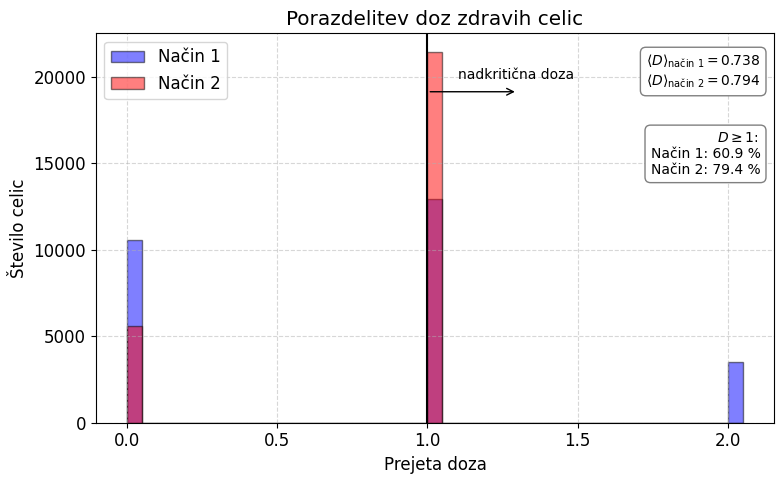
\includegraphics[width=15cm]{Porazdelitev_doz_zdravih_celic.png}
\caption{Porazdelitev doz, ki jih prejmejo zdrave celice v tisoč različnih tumorjih velikosti 15 celic.Podana je tudi povprečna prejeta doza in delež zdravih celic, ki prejme dozo večjo ali enako kritični dozi v obeh načinih reševanja problema. Način 1 je reševanja z minimizacijo doze v zdravem tkivu in način 2 je reševanje z maksimizacijo doze v tumornem tkivu.}
\label{fig:porazdelitev_doz_zdravih_celic}
\end{figure}

\begin{figure}[h!]
\centering
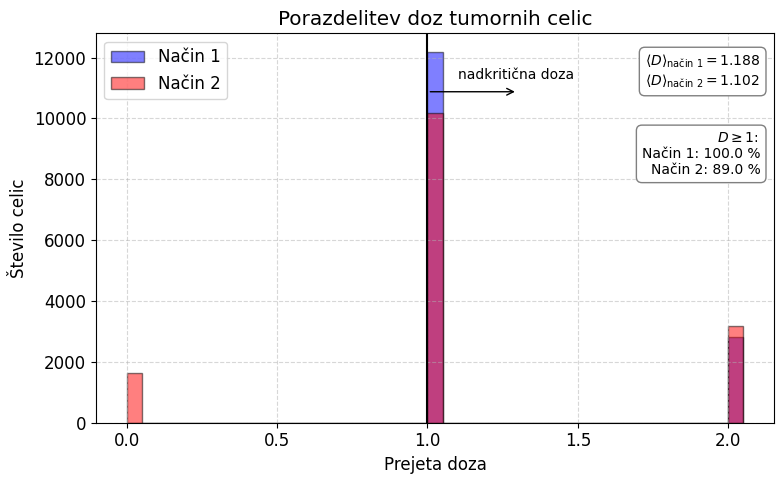
\includegraphics[width=15cm]{Porazdelitev_doz_tumornih_celic.png}
\caption{Porazdelitev doz, ki jih prejmejo tumorne celice v tisoč različnih tumorjih velikosti 15 celic.Podana je tudi povprečna prejeta doza in delež tumornih celic, ki prejme dozo večjo ali enako kritični dozi v obeh načinih reševanja problema. Način 1 je reševanja z minimizacijo doze v zdravem tkivu in način 2 je reševanje z maksimizacijo doze v tumornem tkivu.}
\label{fig:porazdelitev_doz_tumornih_celic}
\end{figure}

\begin{figure}[h!]
\centering
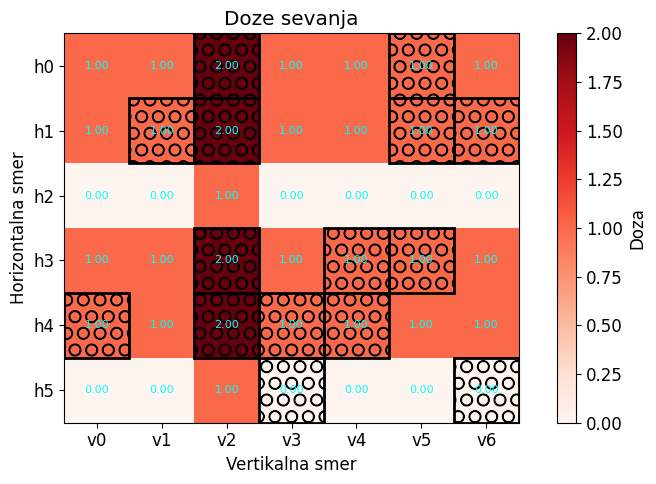
\includegraphics[width=12cm]{primer_tumorja.png}
\caption{Primer tumorja pri katerem z rešitvijo dobljeno z načinom 2 ne obsevamo vseh tumornih celic}
\label{fig:primer_tumorja}
\end{figure}

\subsection{Obsevanost v odvisnosti od velikosti tumorja}

\section{Model eksponentnega curka}

\section{Protonska terapija}

\end{document}
